\documentclass[a4paper,12pt]{exam}
\usepackage{array,amsmath,fancybox,amsfonts,bm}
\usepackage{graphicx,amssymb,wasysym,latexsym,slashed,anysize,subfigure,calc}



%versores: %uso: \uveci\ne\hat{\imath}_{\uvec{i}}+\uvec{j}+\uvec{k}$
	\usepackage{bm}
	\newcommand{\uveci}{{\bm{\hat{\textnormal{\bfseries\i}}}}}
	\newcommand{\uvecj}{{\bm{\hat{\textnormal{\bfseries\j}}}}}
	\DeclareRobustCommand{\uvec}[1]{{%
 	 \ifcsname uvec#1\endcsname
  	   \csname uvec#1\endcsname
  	 \else
   		 \bm{\hat{\mathbf{#1}}}%
   		\fi
									}}


\usepackage{enumitem}
\setenumerate{itemsep=15pt}

%tamaños fuentes extra: 8,9,14,17,20
	\usepackage{extsizes}
	
 %caja bonita
  \usepackage[many]{tcolorbox}
\definecolor{titlebg}{RGB}{80,100,72}
\newtcolorbox{learn}{
  breakable,
  enhanced,
  arc=0pt,
  outer arc=0pt,
  colframe=titlebg,
  colback=titlebg!7,
  overlay unbroken and first={
    \node[
      draw=titlebg,
      fill=titlebg,
      rotate=270,
      anchor=north west,
      text=white,
      font=\bfseries
    ]
    at (frame.north west)  
    {DATOS};
  }
}

%imágenes fundidas texto
\usepackage{wrapfig}

\usepackage{mwe,float,afterpage}

\usepackage{anysize,float}
	%\marginsize{left}{right}{top}{bottom}
    \marginsize{1.25cm}{1.25cm}{1cm}{1cm}
    
    
    
    
%entorno para química: texto y math mode
%\newcommand*\chem[1]{\textup{#1}}
\newcommand*\chem[1]{\ensuremath{\mathrm{#1}}}

%símbolo bonito para qed
\usepackage{amsthm}
	%\newcommand{\mc}[3]{\multicolumn{#1}{#2}{#3}}
\newcommand{\halmos}{\vspace*{-7mm}
	
					\begin{flushright}
						\rule{1mm}{2.5mm} 
					\end{flushright}\vspace*{-6mm}
						
					  }
\renewcommand{\qed}{\halmos}

\usepackage[spanish]{babel}
\usepackage[utf8]{inputenc}
%\usepackage{fancyhdr}
\usepackage{lettrine}

%subrayado y highlight. Tiene que estar detrás de usepackage[color]
\usepackage{soul}
	%\textst{normal} 
	\DeclareRobustCommand{\hlcyan}[1]{{\sethlcolor{cyan}\hl{#1}}} %en cyan!
		%\hl{highlighted text} %uso


%fuentes
	\usepackage[T1]{fontenc}
	\usepackage{mathpazo}

	\usepackage{librebaskerville}

%fancy tables
	\usepackage{booktabs}
	\usepackage[small,centerlast,up]{caption}

	

\usepackage{amssymb,amsmath}
\newcommand{\angstrom}{\mbox{\normalfont\AA}}

\usepackage{graphicx,graphics}
\usepackage{color}
	%	\colorgrids %grids con color
	%	\definecolor{GridColor}{gray}{0.8}
		%grid
%			\setlength{\gridsize}{5mm}
%   			 \setlength{\gridlinewidth}{0.1pt}

%fracciones en texto más elaboradas
	\usepackage{xfrac}

%mejora en la exposición de guarismos
	\usepackage{numprint}
 


%para los entornos de soluciones
\usepackage{mdframed,xcolor,color}
	%uso: 	entorno (begin,end): {mdframed}[backgroundcolor=brown!10] 


\usepackage{everypage,draftwatermark} %Marca de agua
\SetWatermarkText{\parbox{2\textwidth}{\centering 13}}
\SetWatermarkScale{3.8}
\SetWatermarkLightness{0.92}



\pagestyle{headandfoot}

%cabecera
\header{
\includegraphics[scale=.22]{a.png}}       
      {}
       {$FO$ \textbf{B2-{\small dist.}}\\\textbf{abril}{\small 2026}}       
%pie de página

   %enumera en todas menos en la primera
   %\runningfootrule

   %enumera en todas
   %\footrule
   %\footer{}{Página \thepage\ de \numpages}{}
   \footer{}
	{%Página \thepage\ de \numpages
	}
	{%\iflastpage{{\footnotesize \textit{Fin del examen}}}{{\footnotesize \textit{Da la vuelta a la hoja}\ldots}}
	}

	
\begin{document}
	\pagenumbering{gobble}
	
\vspace*{-2ex}

\fbox{\parbox{0.945\linewidth}{\textbf{Nombre y apellidos}:\vspace*{8mm}}}
\vspace{\fill}
		
\begin{learn}
{
% $\triangleright\;G\simeq 6.67\cdot 10^{-11}\;N\,m^{2}\,kg^{-2}$%\hspace{3cm}
 $\triangleright\;c_0\simeq 3\cdot 10^8\;m\,s^{-1} \hspace{1cm} \triangleright\; h\simeq 6.63\cdot 10^{-34}\;J\,s \hspace*{1cm}\triangleright\; e\simeq 1.60\cdot 10^{-19}\;C$
  \vspace{2ex}
  
  $%\triangleright\; 1\;f\!m=10^{-15}\,m\hspace{1.4cm} 
  \triangleright\;\hbar c\simeq 197\;eV\,nm= 197\;MeV\,f\!m,$
  \vspace{2ex}
  
  $\triangleright\;m_ec^2\simeq 511\;keV,\hspace{1.3cm} \triangleright\;m_nc^2\simeq 939.6\;MeV,\hspace{1.3cm} \triangleright\;m_pc^2\simeq 938.3\;MeV,
  \newline
  \triangleright\; m_e\simeq 9.1\cdot 10^{-31}\;kg,\hspace{.65cm}\triangleright\; m_n\simeq1.675\cdot 10^{-27}\;kg,\hspace{.85cm}\triangleright\;m_p\simeq1.672\cdot 10^{-27}\;kg.$
   \vspace{1ex}
   
  $\triangleright\;\epsilon_0\simeq 8.85\cdot 10^{-12}\;C^2\,N^{-1}\,m^{-2}
  %\hspace{.5cm} \triangleright\; \mu_0\equiv 4\pi\cdot 10^{-7}\;N\,A^{-2}
  \hspace{1cm} \triangleright\;K\equiv\frac{1}{4\pi\epsilon_0}\simeq 9\cdot 10^9\;N\,m^2\,C^{-2}.$
  \vspace{1ex}
  
  $\triangleright\;N_A\simeq 6.02\cdot 10^{23}$

  %8,8542·10-12 C2/Nm2
 
  
  
 
% $\triangleright\;c_{\text{sonido}}\simeq 340\;m\,s^{-1}$ \hspace{2.85cm}  $\triangleright\;e^{-1}\simeq 0.37\hspace{5ex} e^{-\sfrac{1}{2}}\simeq 0.61$ 

 %$\triangleright\;G=6.67\cdot 10^{-11}\; N\cdot m^2\cdot kg^{-2}$ 
 %\vspace{1ex}
 
 %$\triangleright\;M_T=5.98\cdot 10^{24}\; Kg$ \hspace{2.8cm}
  %$\triangleright\;R_T=6.4\cdot 10^{6}\; m.$ 
 }
\end{learn}


\newpage
\pagenumbering{gobble}

\vspace*{.1cm}


\begin{enumerate}


	\item Una onda transversal de amplitud $1.5\;cm$ se propaga a lo largo del sentido positivo de la dirección horizontal a una velocidad de $12\;cm\,s^{-1}$. La velocidad máxima de vibración es de $30\;m s^{-1}$ y se sabe que la elongación inicial en el origen es máxima. Determine:
	\begin{itemize}
		\item[a)]  La expresión de la \textbf{elongación} $y(x,t)$.
		\item[b)]  En el punto de máxima elongación asociado a $x=1\,m$ se coloca un zumbador electrónico que emite cada vez que la cuerda lo golpea. ¿Cuál es la \textbf{frecuencia} del sonido emitido por el zumbador?
	\end{itemize}
	\qed
			

	\item 	Una lámpara de luz monocromática de frecuencia $f=5\cdot 10^{15}\,Hz$ emite una radiación de $20\;W$ de potencia. 
			\begin{itemize}
				\item[a)] Suponiendo que la radiación se propaga \textit{en el vacío}, determina su \textbf{longitud de onda y el número de fotones que se emiten por segundo}.
%				\begin{mdframed}[backgroundcolor=brown!10] 
%				A partir de la relación de dispersión para una onda electromagnética libre en el vacío, $c_0=\lambda f$, resulta
%				$$\boxed{\lambda=\frac{c_0}{f}\simeq 6\cdot 10^{-8}\;m.}$$
%				Cada fotón del haz lleva una energía dada por la ecuación de Planck, $E=hf$. Si el haz transporta $N$ fotones y su energía es recogida en un detector durante un intervalo $\Delta t$, resulta que la potencia cumplirá
%				$$P=\frac{\Delta E}{\Delta t}=\frac{Nhf}{\Delta t},$$
%				de donde el número de fotones por unidad de tiempo es $\sfrac{N}{\Delta t}=\sfrac{P}{hf}.$
%				Haciendo números resulta
%				$$\boxed{\frac{N}{\Delta t}=\frac{P}{hf}\simeq 6.0\cdot 10^{18}\;\text{\small fotones por segundo}.}$$
%				\end{mdframed}
				\item[b)] Si en el transcurso de su trayectoria ingresa en un medio homogéneo e isótropo cuyo índice de refracción es $n=1.5$, calcula la \textbf{potencia del haz y su longitud de onda} en este nuevo medio.
%				\begin{mdframed}[backgroundcolor=brown!10] 
%				Si el medio no absorbe energía la frecuencia del haz no varía y por tanto la potencia se conserva, \textit{i.e.} $\boxed{\Delta P=0.}$ Aplicando esta condición a la relación de dispersión obtenemos
%				$$\Delta f=0\rightarrow \frac{c_0}{\lambda_0}=\frac{c}{\lambda}\longrightarrow \lambda=\frac{c}{c_0}\lambda_0=\frac{n_0}{n}\lambda_0=\frac{2}{3}\lambda_0\rightarrow\boxed{\lambda\simeq 4\cdot 10^{-8}\;m.}$$
%				\end{mdframed}
			\end{itemize}
			\qed



%	\item La  Tierra posee dos satélites artificiales, $S_1$ y $S_2$, que describen sendas órbitas circulares de radios $r_1=6798 \;km$ y $r_2=8000\;km$, contenidas en un mismo plano y recorridas en el mismo sentido. En un instante inicial dado, los satélites están alineados con el centro de la Tierra y situados del mismo lado. Calcula:
% 		\begin{itemize}
% 			\item[a)] La relación entre sus velocidades angulares de rotación.
% 			\item[b)] Las vueltas a la Tierra habrá dado $S_2$ cuando $S_1$ haya completado quince vueltas desde el instante inicial.
% 		\end{itemize}
% 		\qed
 		
% 		\begin{mdframed}[backgroundcolor=brown!10] 
%		a) La tercera ley de Kepler para ambos satélites será
%		$$GM_\oplus=\omega_1^2R_1^3=\omega_2R_2^3,$$
%		de manera que
%		$$\frac{\omega_1}{\omega_2}=\left(\frac{R_2}{R_1}\right)^{\frac{3}{2}}\simeq 1.28.$$
%		\end{mdframed}
 			
% 		\begin{mdframed}[backgroundcolor=brown!10] 
%		b) A la vista del apartado anterior podemos deducir que los periodos de los satélites cumplirán 	$\frac{T_2}{T_1}=\left(\frac{R_2}{R_1}\right)^{\frac{3}{2}},$
%		de donde se deduce que $$T_2=\left(\frac{R_2}{R_1}\right)^{\frac{3}{2}}T_1.$$    Hay muchas formas de verlo, pero la más sencilla es entender que el número de vueltas que da un satélite cuando ha pasado un cierto tiempo $\hat t$ es $\frac{\hat t}{T},$
%	    con $T$ el periodo del satélite. Entonces es claro que cuando $S_1$ haya dado 15 vueltas, habrá pasado un tiempo $\hat t=15T_1$ y las vueltas que habrá dado el satélite $S_2$ serán $$\frac{15T_1}{T_2}=\frac{15T_1}{\left(\frac{R_2}{R_1}\right)^{\frac{3}{2}}T_1}=15\left(\frac{R_1}{R_2}\right)^{\frac{3}{2}}\simeq 11.75\text{ vueltas}.$$
%	    
%		\end{mdframed}


	
%	
%	\begin{minipage}{.55\textwidth}
%		\item  Dos cargas eléctricas estáticas positivas e iguales, $+q$, están están separadas una distancia $r$, de acuerdo a la geometría provista por la figura adjunta. Calcule:
%	
%			\begin{itemize}			 
%			 	\item[a)] El campo eléctrico en el punto $A$.
%			 	\item[b)] El trabajo involucrado en desplazar una carga $+Q$ desde $B$ hasta $A$.
%			 \end{itemize}
%		\end{minipage}\hfill
%		\begin{minipage}{.45\textwidth}
%		\vspace*{2ex}
%		
%		\hspace*{.7cm}\def\svgwidth{.75\linewidth}
%			\input{electro.pdf_tex}
%		\end{minipage}
%		\qed
%	

	\item Un foco luminoso emite luz monocromática de longitud $550\;nm$. Se hace incidir 				la luz sobre un metal produciendo la emisión de electrones. La energía mínima de extracción de los 						electrones de la red metálica es de $2.1\;eV$. Calcula:
			\begin{itemize}
				\item[a)] La \textbf{energía} de los fotones incidentes y la \textbf{longitud de onda umbral} para el proceso fotoeléctrico.
				\item[b)] La \textbf{velocidad} del electrón más rápido que se emite. ¿{Son importantes} las \textbf{correciones relativistas}?
			\end{itemize}		 
		\qed	
		
	
	\item Considera una muestra de $1\;g$ del isótopo $^{60}\chem{Co}$, inestable por efecto de la interacción débil, cuyo periodo de semidesintegración tiene una duración aproximada de $5.27\,$ años. Estima:
	\begin{itemize}
		\item[a)] La \textbf{masa} de la muestra pasados $3$ años.
		\item[b)] El \textbf{tiempo} necesario para que la actividad se reduzca a la mitad.
	\end{itemize}
	\qed
		\vspace{3ex}
		
		\begin{minipage}{13cm}
		\item  La barra de la figura se mueve hacia la derecha con una velocidad $v = 2.3\,ms^{-1}$. Las otras dos barras fijas forman un ángulo $\alpha= 45^\circ$ de manera que las tres dan lugar a un circuito cerrado.

En la zona existe un campo magnético externo de módulo $B=0.5\; T$. 
			\begin{itemize}
				\item[a)]  Calcule la \textbf{fem inducida} en el circuito $15\;s$ después de que la barra empiece a moverse.
				\item[b)] Si la resistencia interna circuito en ese instante es $5\,\Omega$, calcule \textbf{el valor y el sentido} de la corriente inducida en $t=15\;s$. 
			\end{itemize}
%			\textit{\textbf{Datos numéricos}:
%			\newline  }
			
\end{minipage}\hfill
\begin{minipage}{4.5cm}
	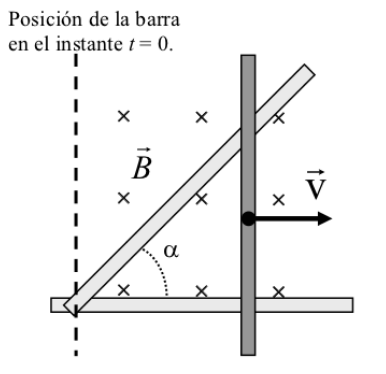
\includegraphics[scale=.5]{cir.png}
\end{minipage}
\qed
		
\end{enumerate}		
 
\end{document}

